\documentclass[12pt]{article}
\usepackage[a4paper, margin=0.75in]{geometry}
\usepackage[document]{ragged2e}
\usepackage{graphicx}
\usepackage{subcaption}
\usepackage{multicol}
\graphicspath{ {./images/} }
\usepackage{enumerate}
\usepackage{framed}
\usepackage{amsmath,amsfonts,amsthm,thmtools,amssymb,mathtools,commath}
\usepackage{physics}
\usepackage{tikz}
\usetikzlibrary{mindmap}
\usepackage{caption}
\usepackage{xcolor}
\usepackage[most]{tcolorbox}
\usepackage{cleveref}


%%%%%%%%%%%%%%%%
%  Definition  %
%%%%%%%%%%%%%%%%
\tcbuselibrary{theorems,skins,hooks}
\newtcbtheorem[number within=subsection]{definition}{Definition}%
{
    % theorem style=definition,
    enhanced,
	before skip=2mm,after skip=2mm, colback=cyan!5,colframe=cyan!80!black,boxrule=0.5mm,
	attach boxed title to top left={xshift=1cm,yshift*=1mm-\tcboxedtitleheight},
	boxed title style={frame code={
					\path[fill=cyan]
					([yshift=-1mm,xshift=-1mm]frame.north west)
					arc[start angle=0,end angle=180,radius=1mm]
					([yshift=-1mm,xshift=1mm]frame.north east)
					arc[start angle=180,end angle=0,radius=1mm];
					\path[left color=cyan!30!black,right color=cyan!30!black,
						middle color=cyan!50!black]
					([xshift=-2mm]frame.north west) -- ([xshift=2mm]frame.north east)
					[rounded corners=1mm]-- ([xshift=1mm,yshift=-1mm]frame.north east)
					-- (frame.south east) -- (frame.south west)
					-- ([xshift=-1mm,yshift=-1mm]frame.north west)
					[sharp corners]-- cycle;
				},interior engine=empty,
		},
	fonttitle=\bfseries,
	title={#2},#1
}{def}


%%%%%%%%%%%%%
%  Theorem  %
%%%%%%%%%%%%%
\tcbuselibrary{theorems,skins,hooks}
\newtcbtheorem[use counter from=definition]{theorem}{Theorem}%
{
    theorem style=plain,
    enhanced,
    colframe=green,
    boxrule=1pt,
    titlerule=0mm,
    toptitle=1mm,
    bottomtitle=1mm,
    fonttitle=\bfseries,
    fontupper=\mdseries\itshape,
    coltitle=green!30!black,
    colbacktitle=cyan!15!white,
    colback=green!10,
    description font=\bfseries\sffamily
}{thrm}


%%%%%%%%%%%%%%
% Corollary  %
%%%%%%%%%%%%%%
 \tcbuselibrary{theorems,skins}
 \newtcbtheorem[use counter from=theorem]{corollary}{Corollary}%
 {
    theorem style=plain,
    enhanced,
    colframe=green,
    frame hidden,
    titlerule=0mm,
    toptitle=1mm,
    bottomtitle=1mm,
    fonttitle=\bfseries,
    fontupper=\mdseries\itshape,
    coltitle=green!30!black,
    colbacktitle=cyan!15!white,
    colback=green!10,
    description font=\bfseries\sffamily
 }{corl}


%%%%%%%%%%%%%
%  Example  %
%%%%%%%%%%%%%
\tcbuselibrary{theorems,skins,hooks}
\newtcbtheorem[number within=section]{example}{Example}%
{
	enhanced,
	breakable,
	colback = gray!5,
	frame hidden,
	boxrule = 0sp,
	borderline west = {2pt}{0pt}{gray},
	sharp corners,
	detach title,
	before upper = \tcbtitle\par\smallskip,
    coltitle=gray!70!black,
	fonttitle = \bfseries\sffamily,
	description font = \mdseries\bfseries
}
{xmp}


%%%%%%%%%%%%%%
%  Exercise  %
%%%%%%%%%%%%%%
\tcbuselibrary{theorems,skins,hooks}
\newtcbtheorem[number within=section]{exercise}{Exercise}%
{
    enhanced,
    breakable,
    colback=black!5,
    colframe=black!30,
    left=0.5em,
    before skip=10pt,
    after skip=10pt,
    boxrule=0pt,
    boxsep=0pt,
    arc=0pt,
    outer arc=0pt,
    borderline west={3pt}{0pt}{black!30},
}{exc}

%%%%%%%%%%
%  Note  %
%%%%%%%%%%
\usetikzlibrary{arrows,calc,shadows.blur}
\tcbuselibrary{skins}
\newtcolorbox{note}[1][]{%
	enhanced jigsaw,
	colback=gray!20!white,%
	colframe=gray!80!black,
	size=small,
	boxrule=1pt,
	title=\textbf{Note:-},
	halign title=flush center,
	coltitle=black,
	breakable,
	drop shadow=black!50!white,
	attach boxed title to top left={xshift=1cm,yshift=-\tcboxedtitleheight/2,yshifttext=-\tcboxedtitleheight/2},
	minipage boxed title=1.5cm,
	boxed title style={%
			colback=white,
			size=fbox,
			boxrule=1pt,
			boxsep=2pt,
			underlay={%
					\coordinate (dotA) at ($(interior.west) + (-0.5pt,0)$);
					\coordinate (dotB) at ($(interior.east) + (0.5pt,0)$);
					\begin{scope}
						\clip (interior.north west) rectangle ([xshift=3ex]interior.east);
						\filldraw [white, blur shadow={shadow opacity=60, shadow yshift=-.75ex}, rounded corners=2pt] (interior.north west) rectangle (interior.south east);
					\end{scope}
					\begin{scope}[gray!80!black]
						\fill (dotA) circle (2pt);
						\fill (dotB) circle (2pt);
					\end{scope}
				},
		},
	#1,
}


\title{
    \textbf{Experiment 3}\\
    \textbf{Observation of Transistor Amplifier Circuits}
}

\author{
    Turja Roy\\
    2108052
}
\date{January 28, 2024}

\begin{document}
\maketitle

\section{Objective}
\begin{enumerate}
    \item To determine voltage, current, and power gain of common emitter amplifier configuration.
    \item To determine voltage, current, and power gain of common base amplifier configuration.
    \item To determine voltage, current, and power gain of common collector amplifier configuration.
\end{enumerate}

\section{Apparatus}
\begin{enumerate}
    \item Transistor (2N3904 n-p-n)
    \item Resistors (1.2 k$\Omega$, 3.6 k$\Omega$, 10 k$\Omega$, 20 k$\Omega$, 220 $\Omega$, 2.2 k$\Omega$, 3.9 k$\Omega$, 3.3 k$\Omega$, 36 k$\Omega$, 1 k$\Omega$)
    \item Capacitors (0.1 $\mu$F, 10 $\mu$F, 47 $\mu$F)
    \item Function generator
    \item DC power supply
    \item Oscilloscope
    \item Breadboard, Wires, Multimeter, etc.
\end{enumerate}

\newpage
\section{Circuit Diagrams}
Below are the circuit diagrams for the three amplifier configurations.
\begin{enumerate}[(a)]
    \item In common emitter amplifier, the input is applied between base and emitter, and the output is taken between collector and emitter. The emitter is common to both input and output.
    \item In common base amplifier, the input is applied between base and emitter, and the output is taken between collector and base. The base is common to both input and output.
    \item In common collector amplifier, the input is applied between base and emitter, and the output is taken between collector and base. The collector is common to both input and output.
\end{enumerate}

\begin{figure}[h!]
    \centering
    \begin{subfigure}{0.45\textwidth}
        \centering
        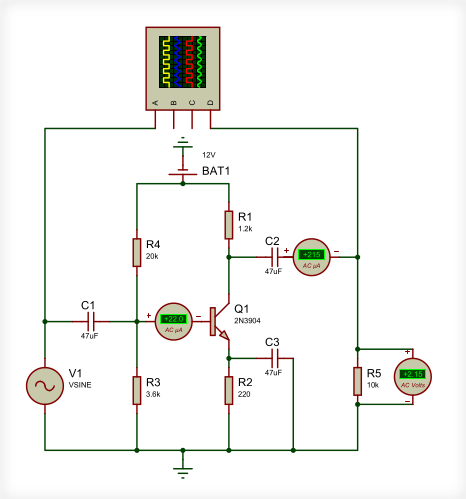
\includegraphics[width=0.9\linewidth]{CE.png}
        \caption{Common Emitter Amplifier}
    \end{subfigure}
    \begin{subfigure}{0.45\textwidth}
        \centering
        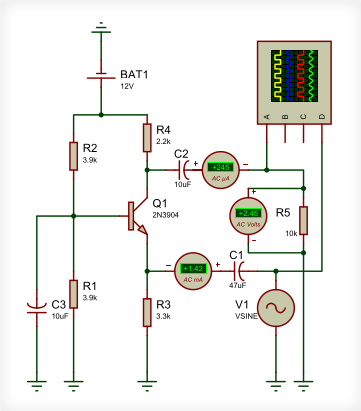
\includegraphics[width=0.9\linewidth]{CB.png}
        \caption{Common Base Amplifier}
    \end{subfigure} \\
    \begin{subfigure}{0.45\textwidth}
        \centering
        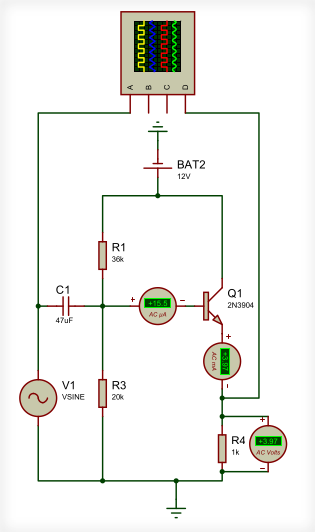
\includegraphics[width=0.6\linewidth]{CC.png}
        \caption{Common Collector Amplifier}
    \end{subfigure}
    \caption{Amplifier Circuit Diagrams}
\end{figure}

\newpage
\section{Result Analysis}
\subsection{Common Emitter Amplifier}
In common emitter amplifier, both voltage gain and current gain are obtained. The voltage gain is higher than the current gain. The amplified output is $180^{\circ}$ phase shifted with respect to the input signal. Below are given the data table (Table 1), the simulated output signal (Figure 2(a)), and the practical output signal (Figure 2(b)).

\bgroup
\def\arraystretch{1.5}
\begin{table}[h!]
    \centering
    \caption{Data table for common emitter amplifier}
    \label{tab:CE table}
    \begin{tabular}{|c|c|c|c|c|c|c|}
        \hline
        \multicolumn{7}{|c|}{\textbf{Theoretical Data}} \\
        \hline
        $V_{in}$ (mV) & $V_{out}$ (V) & $I_{in}$ ($\mu$A) & $I_{out}$ ($\mu$A) & $A_V$ & $A_I$ & $A_P$ \\ \hline
        100 & 2.244 & 22 & 222 & 22.44 & 10.09 & 226.44 \\ \hline\hline
        \multicolumn{7}{|c|}{\textbf{Simulation Data}} \\
        \hline
        $V_{in}$ (mV) & $V_{out}$ (V) & $I_{in}$ ($\mu$A) & $I_{out}$ ($\mu$A) & $A_V$ & $A_I$ & $A_P$ \\ \hline
        100 & 2.92 & 22 & 215 & 29.2 & 9.77 & 285.36 \\ \hline\hline
        \multicolumn{7}{|c|}{\textbf{Practical Data}} \\
        \hline
        $V_{in}$ (mV) & $V_{out}$ (V) & $I_{in}$ ($\mu$A) & $I_{out}$ ($\mu$A) & $A_V$ & $A_I$ & $A_P$ \\ \hline
        30 & 0.8 & 6.1 & 56.7 & 26.67 & 9.3 & 248.31 \\ \hline
    \end{tabular}
\end{table}
\egroup

\begin{figure}[h!]
    \centering
    \begin{subfigure}{0.45\textwidth}
        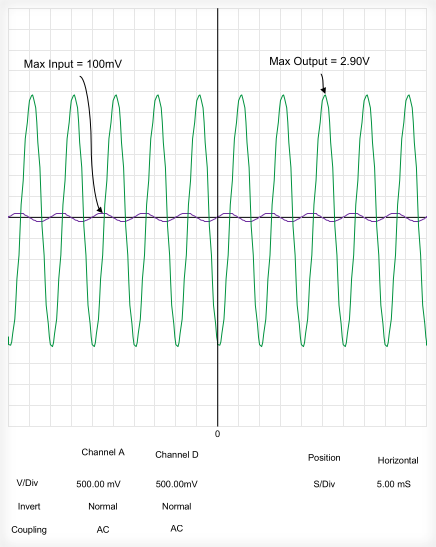
\includegraphics[width=\linewidth]{CE_sim.png}
        \caption{Simulated output signal}
        \label{fig:CE sim}
    \end{subfigure}
    \begin{subfigure}{0.45\textwidth}
        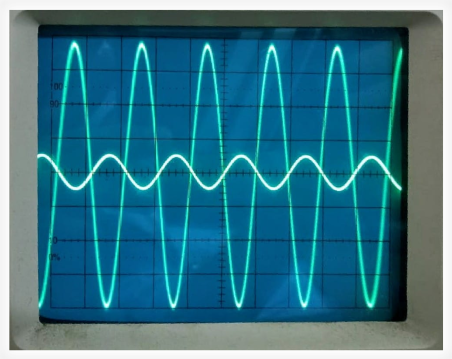
\includegraphics[width=\linewidth]{CE_prac.png}
        \caption{Practical output signal}
        \label{fig:CE prac}
    \end{subfigure}
    \caption{Common emitter amplifier output signal}
    \label{fig:CE signals}
\end{figure}

\subsection{Common Base Amplifier}
In common base amplifier, the current gain is almost equal to 1. The voltage gain is almost same as the common emitter amplifier. Hence, the power gain of a common base amplifier is approximately equal to the voltage gain. Below are given the data table (Table 2), the simulated output signal (Figure 3(a)), and the practical output signal (Figure 3(b)).

\bgroup
\def\arraystretch{1.5}
\begin{table}[h!]
    \centering
    \caption{Data table for common base amplifier}
    \label{tab:CB table}
    \begin{tabular}{|c|c|c|c|c|c|c|}
        \hline
        \multicolumn{7}{|c|}{\textbf{Theoretical Data}} \\
        \hline
        $V_{in}$ (mV) & $V_{out}$ (V) & $I_{in}$ (mA) & $I_{out}$ (mA) & $A_V$ & $A_I$ & $A_P$ \\ \hline
        100 & 11.204 & 6.19 & 6.13 & 112.04 & 0.99 & 110.95 \\ \hline\hline
        \multicolumn{7}{|c|}{\textbf{Simulation Data}} \\
        \hline
        $V_{in}$ (mV) & $V_{out}$ (V) & $I_{in}$ (mA) & $I_{out}$ (mA) & $A_V$ & $A_I$ & $A_P$ \\ \hline
        100 & 2.65 & 1.42 & 1.39 & 26.5 & 0.98 & 25.97 \\ \hline\hline
        \multicolumn{7}{|c|}{\textbf{Practical Data}} \\
        \hline
        $V_{in}$ (mV) & $V_{out}$ (V) & $I_{in}$ (mA) & $I_{out}$ (mA) & $A_V$ & $A_I$ & $A_P$ \\ \hline
        100 & 2.18 & 1.07 & 1.01 & 21.8 & 0.94 & 20.49 \\ \hline
    \end{tabular}
\end{table}
\egroup

\begin{figure}[h!]
    \centering
    \begin{subfigure}{0.45\textwidth}
        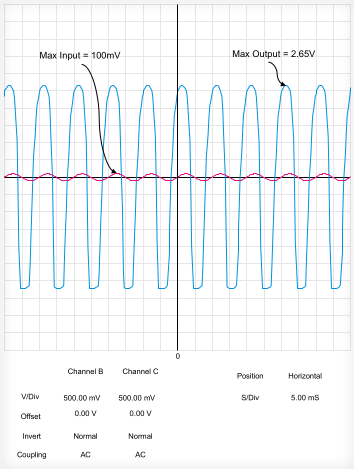
\includegraphics[width=\linewidth]{CB_sim.png}
        \caption{Simulated output signal}
        \label{fig:CB sim}
    \end{subfigure}
    \begin{subfigure}{0.45\textwidth}
        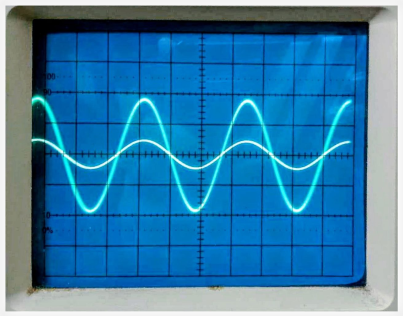
\includegraphics[width=\linewidth]{CB_prac.png}
        \caption{Practical output signal}
        \label{fig:CB prac}
    \end{subfigure}
    \caption{Common base amplifier output signal}
    \label{fig:CB signals}
\end{figure}

\subsection{Common Collector Amplifier}
In common collector amplifier, the voltage gain is less than 1. The current gain is very high. Hence, the power gain of a common collector amplifier is approximately equal to the current gain. Below are given the data table (Table 3), the simulated output signal (Figure 4(a)), and the practical output signal (Figure 4(b)).

\bgroup
\def\arraystretch{1.5}
\begin{table}[h!]
    \centering
    \caption{Data table for common collector amplifier}
    \label{tab:CC table}
    \begin{tabular}{|c|c|c|c|c|c|c|}
        \hline
        \multicolumn{7}{|c|}{\textbf{Theoretical Data}} \\
        \hline
        $V_{in}$ (V) & $V_{out}$ (V) & $I_{in}$ ($\mu$A) & $I_{out}$ (mA) & $A_V$ & $A_I$ & $A_P$ \\ \hline
        2.998 & 2.976 & 263.38 & 2.976 & 0.992 & 11.29 & 11.21 \\ \hline\hline
        \multicolumn{7}{|c|}{\textbf{Simulation Data}} \\
        \hline
        $V_{in}$ (V) & $V_{out}$ (V) & $I_{in}$ ($\mu$A) & $I_{out}$ (mA) & $A_V$ & $A_I$ & $A_P$ \\ \hline
        3 & 2.95 & 170 & 3.97 & 0.983 & 23.35 & 23.01 \\ \hline\hline
        \multicolumn{7}{|c|}{\textbf{Practical Data}} \\
        \hline
        $V_{in}$ (V) & $V_{out}$ (V) & $I_{in}$ ($\mu$A) & $I_{out}$ (mA) & $A_V$ & $A_I$ & $A_P$ \\ \hline
        3 & 2.35 & 135.56 & 4.37 & 0.783 & 32.22 & 25.25 \\ \hline
    \end{tabular}
\end{table}
\egroup

\begin{figure}[h!]
    \centering
    \begin{subfigure}{0.45\textwidth}
        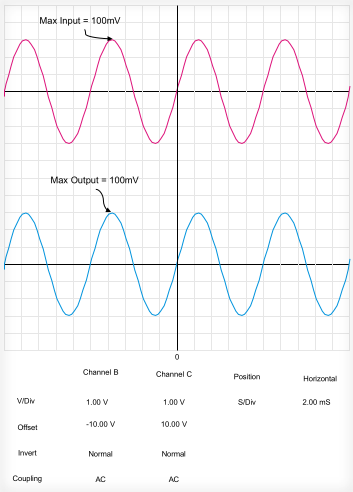
\includegraphics[width=\linewidth]{CC_sim.png}
        \caption{Simulated output signal}
        \label{fig:CC sim}
    \end{subfigure}
    \begin{subfigure}{0.45\textwidth}
        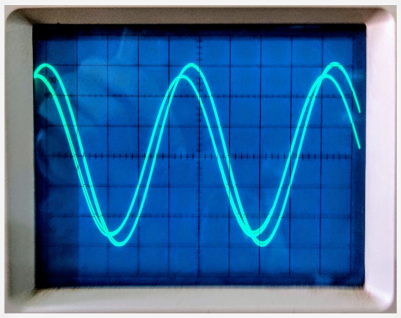
\includegraphics[width=\linewidth]{CC_prac.png}
        \caption{Practical output signal}
        \label{fig:CC prac}
    \end{subfigure}
    \caption{Common collector amplifier output signal}
    \label{fig:CC signals}
\end{figure}

\section{Discussion}
From the experiment results, it can be seen that while the common emitter configuration has both voltage and current gain, the common base and common collector configurations have only voltage gain and current gain respectively. The current gain of common base is nearly 1 and the voltage gain of common collector is nearly 1. The common emitter cofiguration has the highest power gain among the three, followed by common collector and common base configurations respectively.

It was also observed that the output signal of common emitter amplifier is $180^{\circ}$ phase shifted with respect to the input signal. The output signal of common base amplifier is in phase with the input signal. The output signal of common collector amplifier is slightly out of phase with respect to the input signal.

The discripancies between the theoretical, simulated, and practical data can be attributed to different reasons. The theoretical data was calculated using ideal values, while the practical data was obtained using real components that have some tolerances. Temperature plays a role in BJT circuits since BJTs are more susceptible to thermal runaway. The errors could have been minimized by performing the experiment under a much more controlled environment.

\end{document}
